
%NB: I need to fix some of the formatting
% at the moment it only seems to allow one figure or table per page and puts various text blocks in between
% Probably something in the mythesis style template

\chapter{Data collection}
\label{chap:methods}

\section{Introduction}

The analyses in chapters %\chapref{}, \chapref{}… 
use morphological and ecological data sets which I compiled for xx specimens representing xx species of small mammals. This chapter describes how the data were collected and checked for errors. First I outline how I compiled my morphological data set from museum specimens and secondly I describe the sources which contributed to my ecological dataset. Subsequent chapters will refer to both of these data sources but I will only describe the methods I used for their creation in detail here. Other methods I used which have specific relevance to subsequent chapters are described in those chapters.   
%####################################################

\section{Study species}
I collected morphological measurements of xxx species from  four mammalian orders; Afrosoricida, Erinaceomorpha, Soricomorpha and Notoryctemorphia comprising seven families of mammals; tenrecs (Tenrecidae), golden moles (Chrysochloridae), hedgehogs and gymnures(Erinaceidae), shrews (Soricidae), solenodons (Solenodontidae), moles and desmans(Talpidae) and marsupial moles (Notoryctidae).
My aim was to include measurements of all tenrecs and their sister taxa, golden moles.  For my  comparative species from other mammalian orders, I chose a random sample of xx taxa which have been previously identified as convergent with tenrecs \citep[e.g.][]{Gould1966, Symonds2005, Poux2008, Olson2013}. I followed the taxonomy in Wilson and Reeder's Mammal Species of the World (MSW) \citeyearpar{Wilson2005}. I used phylogenies for each order to select, at random, species representing the main sub-branches of each order which also represented the morphological diversity of that order. For example, within the Soricomorpha, I included both species of \textit{Solenodon} but only xx (out of a total of xx) species of \textit{Crocidura} as the former genus represents a separate subgroup to the rest of the order. 
%*****************************************
%Come back and rephrase this setion
%*****************************************
%####################################################
\section{Taxonomy}

Although MSW is a comprehensive mammalian taxonomic reference, it does not include some known species. For example, Wilson and Reader \citeyearpar{Wilson2005} record 30 species of tenrec but more recent studies indicate that there are now 34 recognised species of tenrec \citep{Olson2013}. The additional species belong to the shrew tenrec (\textit{Microgale}) genus and represent either recognition of cryptic species boundaries \citep{Olson2004} or discovery of new species \citep{Goodman2006, Olson2009}. Only one of these four recent additions to the \textit{Microgale} genus, \textit{M. jobihely}, was present in museum collections and therefore I could not include the three other newly recognised species in my analyses.

As MSW does not include all known species, I used the International Union for the Conservation of Nature \citep{IUCN2012} as an additional reference for the taxonomy and species diversity of each group. Table \ref{tab:species.measured} outlines the number of species I measured from each family and how this sample relates to the overall number of species in that group as recorded by both MSW and the IUCN.

%Species.measured table

\begin{table}[h]
\caption[Summary of species measured] %this appears in the table of contents
{The number of species I measured in each family compared to the total number of species in that family according to two sources; \citep{Wilson2005} and \citep{IUCN2012}}
%Species.measured table
%To get the number measured for each Family, I counted the number of unique species in my Tb_Taxonomy Access table for that family
%So it's the number of species measured overall but that doesn't necessarily mean that I have the same number in every data set
%I didn't count the _sp. specimens as separate species

%I took out the reference to the IUCN because it seems to only list species that are threatened/endangered rather than a full list of all species in a family

\begin{tabular}{p{3.4cm}p{3cm}p{2cm}p{2cm}p{2cm}}

\hline
\textbf{Order} & \textbf{Family} & \textbf{Measured species} & \textbf{Total species} & \textbf{Coverage} \\
\hline
%----------------------------------------------------
Afrosoricida & Tenrecidae & 31 & 34 & 91 \% \\
%-------------------------------------------------
Afrosoricida & Chrysochloridae & 12 & 21 & 57 \% \\
%----------------------------------------------------
Erinaceomorpha & Erinaceidae & 16 & 24 & 67 \% \\
%----------------------------------------------------
Soricomorpha & Soricidae & 22 & 376 & 5.8 \% \\
%----------------------------------------------------
Soricomorpha & Solenodontidae & 2 & 4 & 50 \% \\
%----------------------------------------------------
Soricomorpha & Talpidae & 15 & 39 & 38 \% \\
%----------------------------------------------------
Notoryctemorphia & Notoryctidae & 1 & 2 & 50 \% \\
%-----------------------------------------------
\hline

\end{tabular}

%*There are now 34 recognised tenrec species \citep{Olson2013}
\label{tab:species.measured}
\end{table}

%####################################################
\section{Morphological data set}
To construct my morphological data set, I used museum specimens of my study species housed at five different institutions. I compiled morphological data using two complementary approaches; linear measurements using calipers and 2D landmark-based geometric morphometrics.

\subsection{\normalfont{Museums visited}}

I measured and photographed the skulls, limbs and skins of tenrecs and the species they convergently resemble using the collections of five different museums; the Natural History Museum London (NHML), the Smithsonian Institute Natural History Museum (SI), the American Museum of Natural History (AMNH), Harvard’s Museum of Comparative Zoology (MCZ) and the Field Museum of Natural History (FMNH), Chicago. Between January and September 2013, I spent 9 weeks working in these collections and collected data from xxx skulls, xxx limbs and xxx skins of xxx species. 

\subsection{\normalfont{Museums label data}}
I recorded all the data on the specimen labels including any handwritten or printed notes which had been added by other users of the collection. The label data included the museum specimen ID number, genus, species, sex, collector’s name, the date and location of where the specimen was collected. Some of the labels attached to skins had additional information such as the body, tail, hind foot and ear lengths as well as the body mass of the live individual. 
The level of detail recorded on the labels varied considerably (figure \ref{fig:museum.labels}). For example recently collected specimens were more likely to have detailed information about the collection location, and some specimens did not have even basic information such as the sex recorded. 

%Museum label pictures

\begin{figure} 
  \centering
  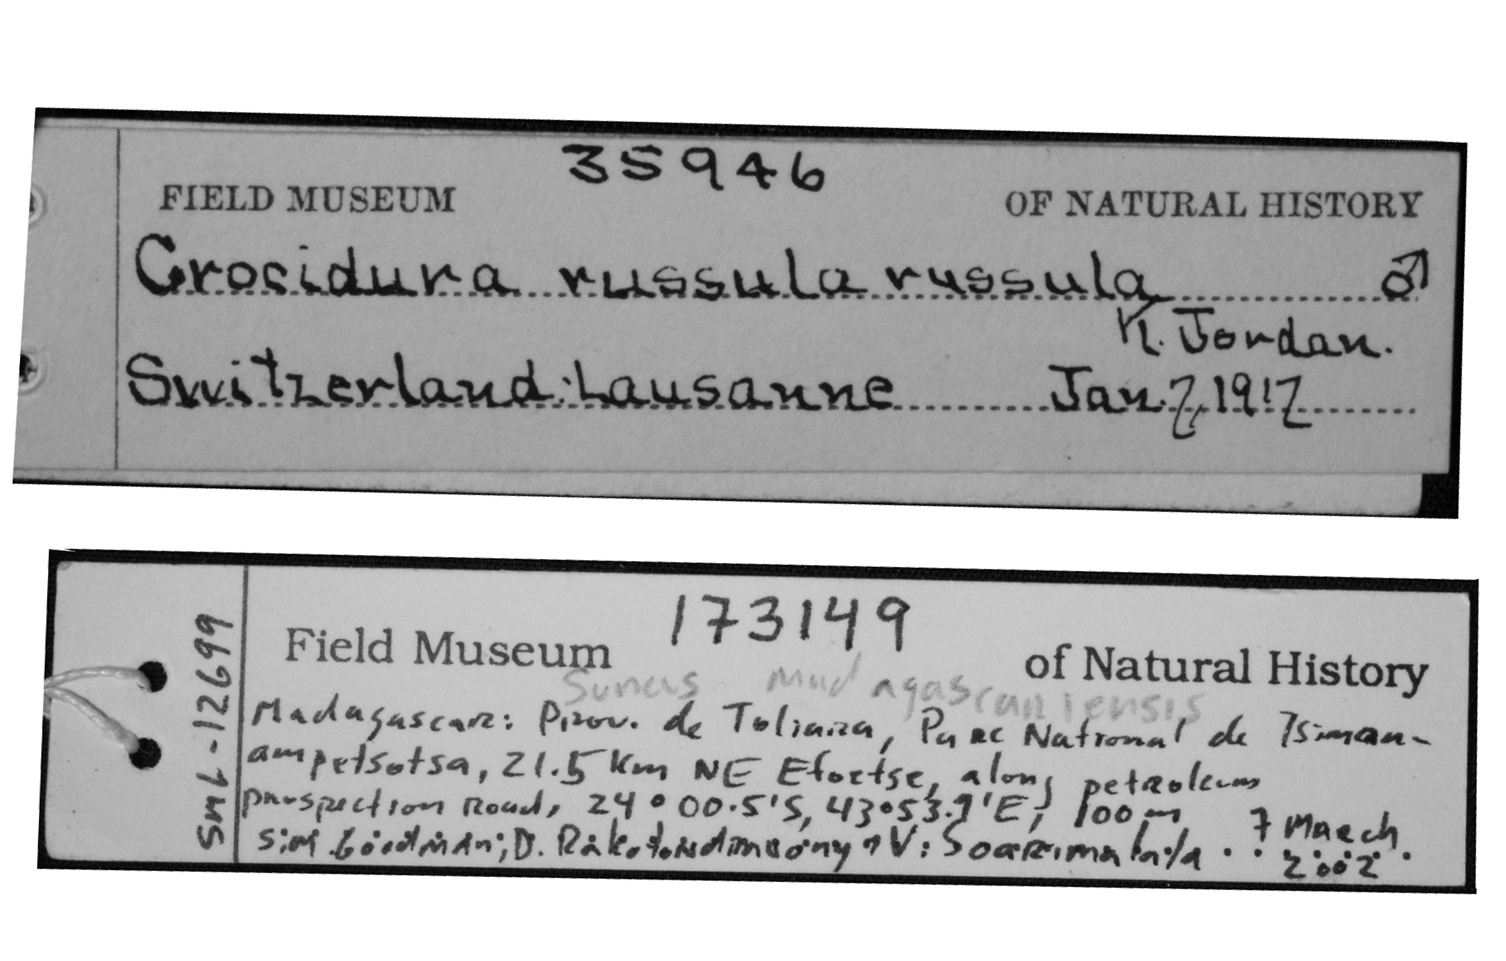
\includegraphics[width = 15cm, height = 15cm, keepaspectratio=true]{Methods/figures/labels.png}
    \caption[Examples of museum labels]%this is what appears in table of contents
    {Examples of the variation in the detail of information which is available from museum labels}%this is under the figure
  \label{fig:museum.labels}
  \end{figure}
  
%------------------------------------------------
\section{Linear measurements}

Using a 15mm digital calipers (Mitutoyo Absolute digimatic calipers), I took 20 measurements of the skulls and mandibles (table \ref{tab:sk.measurements}) and 19 measurements of the limbs (table \ref{tab:limb.measurements}). My choice of which measurements to include was based on three main criteria; 1) their relevance to biological and ecological traits such as diet specialisation and locomotory adaptation, 2) their usefulness for assessing the overall shape and size of the specimen and 3) the ease with which they could be repeated both within and among specimens from different species. 
Figures x-x depict the linear measurements of skulls and figures xx show the limb measurements.

%******************************
%I need to put in diagrams here
%I need to fill in these tables
%******************************************
% Skull and mandible measurements

\begin{table}[h]
\caption[Description of the skull and mandible measurements]
		{Skull and mandible measurements}% add to this caption
%Skull measurements

\begin{tabular}{lp{3.5cm}p{9.75cm}}
\hline
\textbf{Abbreviation} & \textbf{Measurement} & \textbf{Description}\\
\hline
CB & Condylobasal length & Total skull length from the front of the premaxillary  bones to the rear of the occipital condyles, measured from below \\
%-------------------------------------------
PL & Palate length & Maximum length of the palate from the anterior of the pre-maxilla to the posterior of the hard palate\\
%----------------------------------------------
TR & Tooth row length & From the front of the alveolus of the first incisor to the rear of the alveolus of the last molar on the same side\\
%----------------------------------------------
PWa* & Palate width anterior & Width across the palate measured between the posterior, outer-most points of the alveoli of the first pair of teeth\\
%I had to modify this measurement slightly for some species: when there was a row of anterior incisors which stretch across the front of the palate (e.g. Euroscaptor klossi SI_261090) then I measured PWa as the width across from back of the row of the incisors on either side (i.e. just in front of the canines) 
%----------------------------------------
maxPW & Maximum palate width & Measured at the widest point of the palate\\
%--------------------------------------------
IncisorH* & Incisor height & Maximum height of the first incisor on the right\\
%----------------------------------------
ZW & Zygomatic width & Maximum width between the zygomatic arches (measured within the arches from below the skull)\\
%---------------------------------------
MX & Maxilla width & Width between the maxillary bones, measured from above the skull. Species with zygomatic arches; width from the innermost connection between the anterior of the arch and the skull. No arches; width between the anterior skull constrictions.\\ 
%---------------------------------------
SQ & Squamosal width & Width between the squamosal bones, measured from above the skull. Species with zygomatic arches; width from the innermost connection between the posterior of the arch and the skull. No arches; width between the posterior skull constrictions \\
%-------------------------
OL & Orbit length & Longitudinal length of the orbit opening measured along the edge of the skull from the maxilla to the squamosal. \\
%------------------------------
IFD* & Interorbital foramen width & The maximum (vertical) diameter of the right interorbital foramen\\
%-----------------------------------------------
IFW & Interorbital foramen width & Maximum width across the skull between the two interorbital foramina, measured from above\\
%-------------------------------
IFcanal* & Interorbital foramen canal & Length of the right IF canal measured between the anterior and posterior openings from above\\
%---------------------------------
BW & Braincase width & Width across the braincase at the widest point of the skull\\
%---------------------------------
SkH & Skull height & Perpendicular height from the highest point on the braincase to the base of the skull\\



\hline
\end{tabular}
\label{tab:sk.measurements}
\end{table}

%-----------------------------------------
% Limb measurements
\begin{table}[h]
\caption[Description of the limb measurements]
		{Limb measurements} % add to this caption
%Limb measurements


\begin{tabular}{lp{3.5cm}p{9.75cm}}
\hline
\textbf{Abbreviation} & \textbf{Measurement} & \textbf{Description}\\
\hline
Inn & Innominate length & Maximum longitudinal length of the pelvic bone measured in a straight line from the anterior tip to the posterior curve \\ 
%-----------------------------------
Obt & Obturator foramen & Maximum diameter of the opening in the pelvic bone \\
%-----------------------------------
FemL & Femur length & Length of the bone excluding the femoral head (i.e. length of the bone without the joint area)  \\
%-----------------------------------
FemD* & Femur diameter & Minimum width across the shaft of the bone \\
%-----------------------------------
TibL & Tibia length & Maximum longitudinal length of the tibia  \\
%-----------------------------------
TibU & Tibia unfused length & Length of the tibula which is not fused with the fibula \\
%-----------------------------------
TibD* & Tibia diameter & Minimum diameter across the shaft of the tibia bone \\
%-----------------------------------
Foot & Foot length & Maximum length of the entire foot (heel to longest toe) \\
%-----------------------------------
Toe & Toe length & Length of the longest toe bone (just the phalange bone up to the metatarsal joint) \\
%-----------------------------------
ScapL & Scapula length & Perpendicular length of the scapula from the curved end to the anterior point  \\
%-----------------------------------
ScapW & Scapula width & Maximum perpendicular width across the bone \\
%--------------------------------
HumL & Humerus length & Maximum length of the bone. In golden moles (L-shaped humerus): diagonal distance between the two ends of the bone  \\
%-------------------------------
HumLvert & Humerus length vertical & Only for golden moles with L-shaped humerus: length of the vertical (longer) side of the bone \\
%-------------------------------
HumLhori & Humerus length horizontal & Only for golden moles with L-shaped humerus: length of the horizontal (shorter) side of the bone \\
%-----------------------------------
HumD* & Humerus diameter & Minimum diameter across the shaft of the humerus \\
%-----------------------------------
UlnL & Ulna length & Length of the bone from the posterior tip to the wrist joint \\
%-----------------------------------
RadL & Radius length & Length of the bone from the posterior tip to the wrist \\
%--------------------------------
UlnD* & Ulna diameter & Minimum diameter across the ulna \\
%-------------------------------
RadD* & Radius diameter & Minimum diameter across the radius \\
%----------------------------
Hand & Hand length & Maximum length of the entire hand (wrist to longest finger) \\
%------------------------
Finger & Finger length & Length of the longest finger bone (to the metatarsal joint) \\
%---------------------
\hline

\end{tabular}
\label{tab:limb.measurements}
\end{table}

%*****************************
%Figures of the measurements
%****************************

I took each linear measurement three times, cycling through all 20 skull or 19 limb measurements then repeating the cycle to avoid measuring the same variable twice in a row. Small measurements (<2 mm) are particularly prone to high error rates \citep{Cardini2008}. Therefore, I took five separate replicates of some of the variables which were most prone to errors (marked with PUT IN SYMBOL in tables \ref{tab:sk.measurements} and \ref{tab:limb.measurements}). These included four of the skull measurements (PWa, IncisorH, IFD and IFcanal) and five of the limb measurements (FemD, TibD, HumD, UlnD, RadD). 
Five replicates should give a more reliable median value because even if there are one or two outlying measurements there should be at least three replicates which are in close agreement.
%####################################################

\section{Landmark morphometrics}
\subsection{\normalfont{Photographic setup}}
In order to get 2D landmarks for my specimens, I first had to photograph them. I used photographic copy stands consisting of a camera attachment with an adjustable height bar, a flat stage on which to place the specimen and an adjustable light source to either side of the stage. I used the copy stands that were available at each museum which differed in how the camera height was adjusted and in the light sources available.
To take the light variability into account, on each day I took a picture of a white sheet of paper and used the custom white balance function on the camera to set the image as the baseline “white” measurement for those particular light conditions.

\subsection{\normalfont{Photographing specimens}}
I photographed the specimens with a Canon EOS 650D camera fitted with either an EF 100mm f/2.8 Macro USM lens (skulls and limbs) or EFS 18-55mm lens (skins). I used a remote control (h\"ahnel Combi TF) to take the photos to avoid shaking the camera and distorting the images. I photographed the specimens on a black material background. I placed the light source from the top left-hand corner of the picture and positioned a piece of white card on the bottom right side of the specimen which reflected the light back onto the specimen and minimised any shadows (figure \ref{fig:camera} below).

%----------------------------------------------
%Camera picture
\begin{figure}[h] 
  \centering
  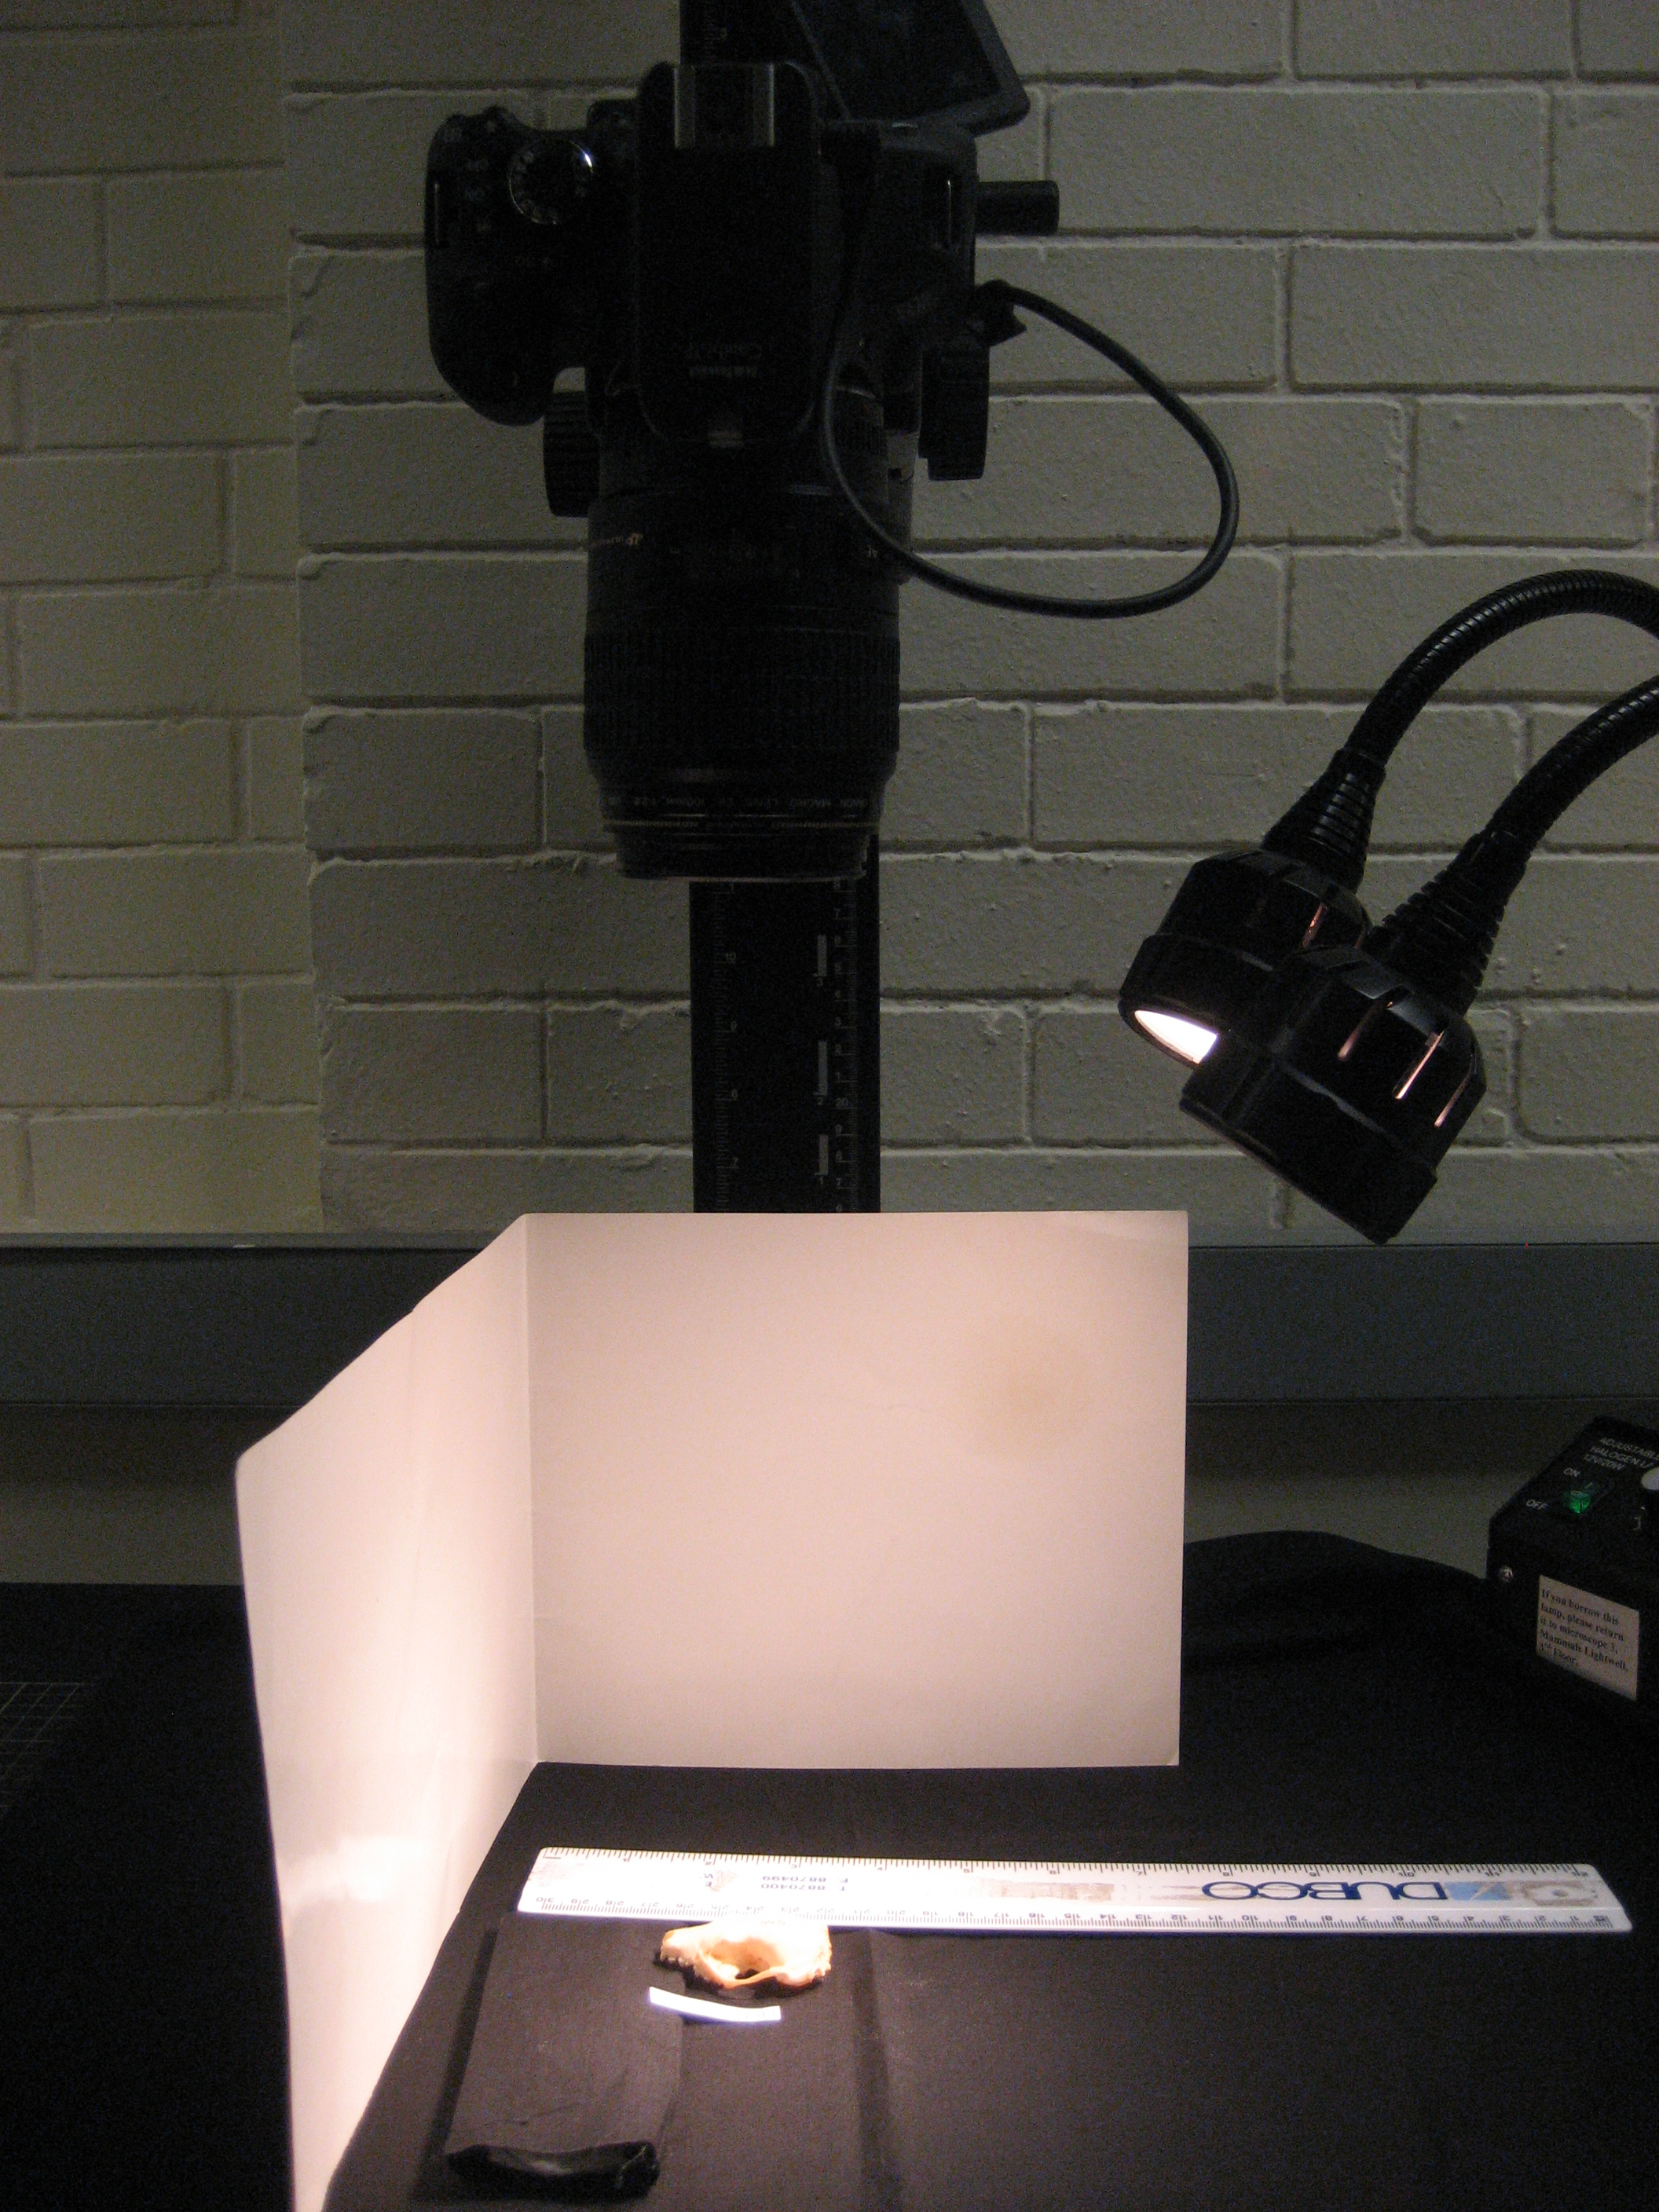
\includegraphics[width=12cm, height=12cm, keepaspectratio=true]{Methods/figures/camera.jpg}
    \caption[Photographic set up]%this is what appears in table of contents
    {Photographic set up for taking images of my skulls. The camera (above centre) is fitted to a copy stand, the light source is directed from the top-left corner of the image and the white card reflects the light back onto the skull. }%this is under the figure
  \label{fig:camera}
  \end{figure}
%-------------------------------------------------
I made small bean bags (12 x 5cm) from the same black material as the background and filled them with plastic beads. I used these bags as necessary to hold the specimens in position while being photographed. For example, when taking pictures of the lateral view of skulls, I placed one bean bag under the nose of the skull and another bag lying along the top (cranial) side of the skull to ensure that the side I was photographing lay in a flat plane relative to the camera and did not tilt in any direction. 
I used the grid-line function on the live-view display screen of the camera to position the specimens in the centre of each image. 

\subsection{\normalfont{Skulls}}
I photographed the skulls in three views; dorsal (top of the cranium), ventral (underside of the skull with the palate roof facing uppermost) and lateral (right side of the skull). I also photographed the outer (buccal) side of the right mandible. When the right side of either the skull or mandibles were damaged or incomplete, I photographed the left sides and later reflected the images so that they could be compared to pictures of the right sides \citep[e.g.][]{Barrow2008}.

%Probably need a disclaimer somewhere about not being interested/ worried about bilateral asymmetry and also a quick test.

\subsection{\normalfont{Limbs}}
Initially, I tried to take pictures of the limbs in similar orientations to the skulls (dorsal, ventral and lateral). However, there was considerable variation in how the limbs were preserved. For example, some limbs were still articulated while others had fragmented bones. It therefore proved impossible to place the limb bones in consistent orientations that would be comparable across species. Similarly, the small size of some limbs, combined with the frequently incomplete nature of postcranial museum collections, made landmark-based morphometric analyses of any limb pictures impractical. Therefore, I photographed the fore- and hind-limb bones in outer (the side facing away from the rest of the body) and inner (the side facing in towards the centre of the body) views for reference purposes only.

\subsection{\normalfont{Skins}}
As I was limited by the maximum camera height available on the copy stands, most skins were too large to be photographed with the 100mm macro lens. Therefore, I used an EFS 18-55mm lens to take pictures of the skins. I photographed skins in the same three orientations as the skulls; dorsal (the upper surface of the animal), ventral (the belly side of the skin) and lateral (right flank of the animal with the skin held in position using bean bags). The dorsal and ventral views give very approximate estimates of the overall body shape of the animal. The lateral views are less biologically relevant since the taxidermic process is unlikely to produce specimens which represent the true body height of the animal.

\subsection{\normalfont{Saving and processing images}}
Photographs were captured and saved in a raw file format. Before using the pictures for morphometric analyses, I converted the raw files to binary (grey scale) images and re-saved them as TIFF files. The black and white pictures were more useful for later analyses since I was not interested in including any colour comparisons and it is easier to see some biological features in binary images. TIFF files were the most appropriate to use for my morphometric analyses as they are uncompressed (in comparison to JPEG) images and therefore there is less chance of any picture distortions which may affect later analyses \citep{HERC2013}.

\subsection{\normalfont{Landmark placement on images}}
%I need a general “this is morphometrics” overview at some stage; it might fit in here?

I conducted geometric morphometric analyses of my skull and mandible photographs. I used a combination of landmark and semilandmark analysis approaches to assess the shape variability of the specimens. In contrast to detailed morphometric studies of single taxa (e.g. Refs), the interspecific and comparative nature of my work limited the number of points which could be reliably identified as landmarks in all species….
%*******************************
%Tidy up this section
%********************************
I used the TPS software suite \citep{Rohlf2013} to digitise landmarks and curves on my pictures. I set the scale on each pictures individually to standardise for the different camera heights I used when photographing my specimens. I created separate data files for each of my morphometric analyses (three views of skulls and lateral view of mandibles). I digitised landmarks and semilandmark points on each picture individually.

When combining landmark and semi-landmark approaches, there is a potential problem of over-sampling the curves (REFS). To determine the number of semilandmark points required to adequately summarise the curves in my data sets,  I followed the method outlined by MacLeod \citeyearpar{MacLeod2012}. For each data set I chose a random selection of pictures of specimens which represented the breadth of the morphological data (i.e. specimens from each sub-group of species).  I drew the appropriate curves on the each specimen and over-sampled the number of points on the curves. I measured the length of the line and regarded that as the 100\%, true length of that outline. I then re-sampled the curves with decreasing numbers of points and measured the length of the outlines. I calculated the length of each re-sampled curve as a percentage of the total length of the curve and then found the average percentage length for across all of the specimens in my test file. I continued this process until I found the minimum number of points that gave a curve length which was at least 96\% accurate.  I repeated these curve-sampling tests for each analysis to determine the minimum number of semilandmark points which would give accurate representations of morphological shape.
After creating my files with the landmarks and semilandmarks placed on each picture, I built sliders files \citep{Zelditch2012} to specify which points should be treated as semilandmarks in further analyses. After landmarking and building sliders files, I used R v3.02 \citep[R Development Core][]{Team2013} for all subsequent statistical analyses.

Here I summarise the landmarks and curves which I used on each of my different sets of pictures. For landmarks which are defined by dental structures, I used published dental formulae \citep{Nowak1983, MacPhee1987, KnoxJones1992, Marshall1996, Nagorsen2002, Goodman2006, Asher2008, ADW2013} where available to identify the number and type of teeth in each species.

%***************************************************************
%(I’ll need to put in pictures showing the landmarks for each set of photos- do another photo shop job on pictures and then add points to that.)
%**************************************************************
\subsection{\normalfont{Skulls: ventral view}}

Most of the landmarks in this view are concentrated around the dentition and palate of the animals. I placed 13 landmarks and drew one outline curve (resampled to 60 semilandmark points) around the back of the skull between landmarks 12 and 13 (figure X). The high variability of my species’ basi-cranial region and difficulties associated with identifying developmentally or functionally homologous points precluded designation of additional landmarks towards the back of the skulls. Table \ref{tab:skvent} outlines the descriptions of the landmarks I placed on the ventral pictures.

% Skulls ventral landmarks

\begin{figure}[h] 
  \centering
  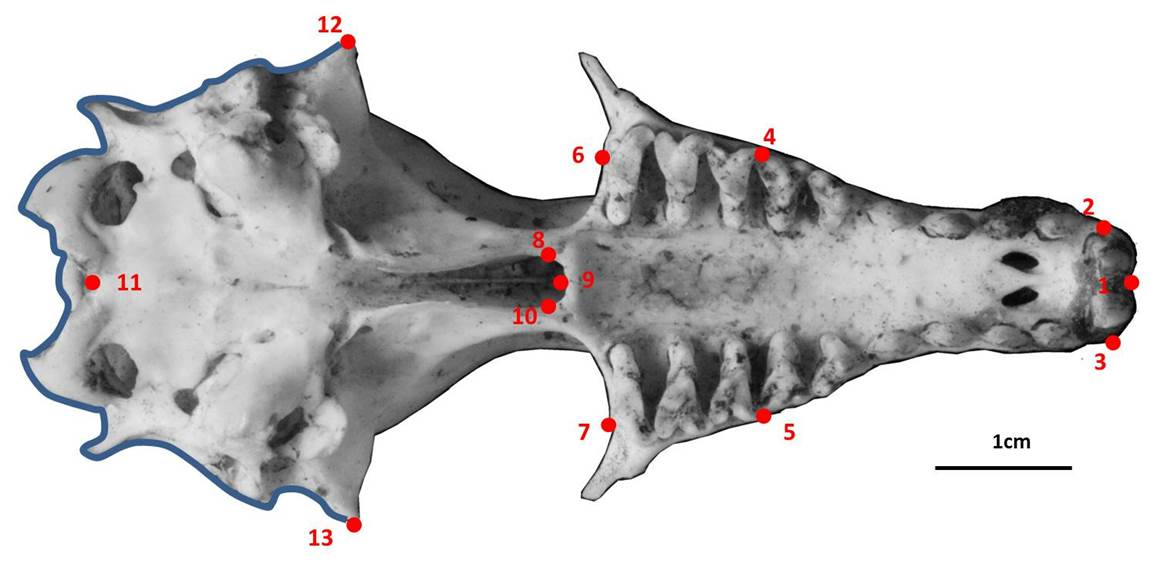
\includegraphics[width=12cm, height=12cm, keepaspectratio=true]{Methods/figures/skvent_landmarks_pot_vel.jpg}
    \caption[Skulls: ventral landmarks]%this is what appears in table of contents
    {Landmarks (red) and curve (blue) for the ventral skull pictures, further descriptions in table \ref{tab:skvent}. The specimen is a giant otter shrew tenrec, \textit{Potamogale velox}, NHML 1934.6.16.2}
  \label{fig:skvent_landmarks}
  \end{figure}

\begin{table}[h]
\caption[Skulls: ventral landmarks]
		{Descriptions of the landmarks (points) and curves (semilandmarks) for the skulls in ventral view (figure \ref{fig:skvent_landmarks})} 
%SkVent landmarks
\begin{tabular}[t]{p{0.2\textwidth} p{0.75\textwidth}}		
\hline
\textbf{Landmark} & \textbf{Description} \\
\hline
%--------------------------------------
1 & Anterior point of the palate\\
%--------------------------------------
2 + 3 & Posterior, lateral extremity of the right (2) and left (3) incisor\\
%--------------------------------------
4 + 5 & Anterior, outer point of the first molar on the right (4) and left (5)\\
%--------------------------------------
6 + 7 & Posterior, outermost point of the last molar surface on the right (6) and left (7) \\
%--------------------------------------
8 & Widest point of the curve of the palatine on the right side\\
%--------------------------------------
9 & Posterior point of the palatine in the midline\\
%--------------------------------------
10 & Widest point of the curve of the palatine on the left side\\
%--------------------------------------
11 & Anterior of the occipital foramen in the midline\\
%--------------------------------------
12 + 13 & Widest (extreme lateral) point of the braincase on the right (12) and left (13)\\
%--------------------------------------
Curve*  & Outline of the back of the skull (between landmarks 12 and 13), 60 points \\
%------------------------------------------------------------
\hline
\end{tabular}
\label{tab:skvent}
\end{table}
%==================================================================
\subsection{\normalfont{Skulls: lateral view}}
I placed nine landmarks on the lateral pictures (see figure \ref{fig:sklat_landmarks} below) and also drew two semilandmark curves between landmarks 7 and 8 to represent the shape of the back of the skull (resampled to 20 semilandmark points) and landmarks 8 and 1 (resampled to 15 semilandmark points) down the midline of the nose to represent the shape of the top of the skull. Table \ref{tab:sklat} describes my definitions for each of the landmark points.
For specimens that were damaged on their right side we reflected photographs of the left lateral side of the skull so that all pictures would be in the same orientation.
I originally tried to include more landmarks around the infraorbital foramina (IF) as a crude measure of facial sensitivity and because the IF area is correlated with ecotypes \citep{Crumpton2012}. However, it proved impossible to see the boundaries of the IF in many species and single landmark points could not represent the shape of the full foramina. 

%Sklat diagram and landmarks description
\begin{figure}[h] 
  \centering
  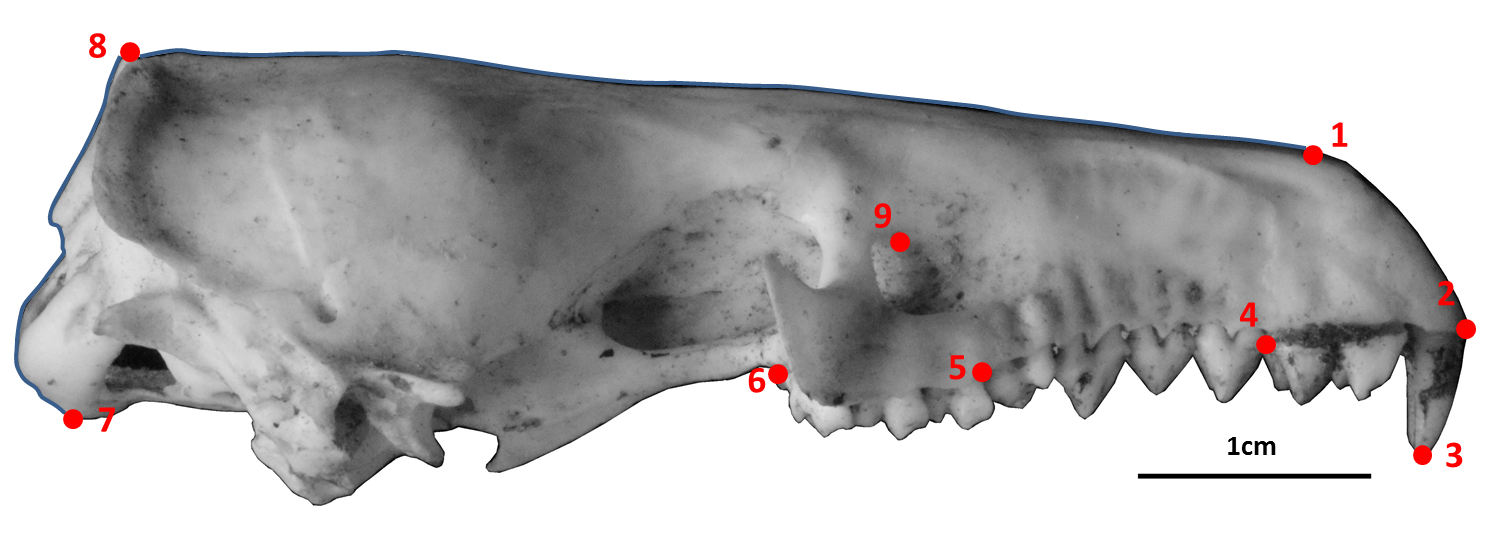
\includegraphics[width=12cm, height=12cm, keepaspectratio=true]
  {Methods/figures/sklat_landmarks_pot_vel.png}
    \caption[Skulls: lateral landmarks] {Landmarks (red) and curve (blue) for the lateral skull pictures, further descriptions in table \ref{tab:sklat}. The specimen is a giant otter shrew tenrec, \textit{Potamogale velox}, NHML 1934.6.16.2}
  \label{fig:sklat_landmarks}
  \end{figure}

\begin{table}[h]
\caption[Skulls: lateral landmarks]
		{Descriptions of the landmarks (points) and curves (semilandmarks) for the skulls in lateral view (see Figure X.} 
%Sklat landmarks

\begin{tabular}[t]{p{2cm} p{12cm}}		
\hline
\textbf{Landmark} & \textbf{Description} \\
\hline
%--------------------------------------
1 & Anterior, upper tip of the nasal bone\\
%--------------------------------------
2 & Anterior of the alveolus of the first incisor\\
%--------------------------------------
3 & Lowest point of the first incisor\\
%--------------------------------------
4& Posterior of the alveolus of the last incisor \\
%--------------------------------------
5 & Anterior tip of the alveolus of the first molar\\
%--------------------------------------
6 & Posterior tip of the alveolus of the last molar\\
%--------------------------------------
7 & Lowest point of the basi-occipital (base of the back of the skull)\\
%--------------------------------------
8 & Highest point of the braincase\\
%--------------------------------------
9 & Highest point of the infraorbital foramen\\
%--------------------------------------
\hline
\textbf{Curve A} & Between points 7 and 8  \\
(20 points)& Back of the skull from the lowest to highest points\\
%------------------------------------------------------------
\textbf{Curve B} & Between points 8 and 1  \\
(15 points)&From the highest point of the braincase to the front of the nasal \\
%------------------------------------------------------------
\hline
\end{tabular}
\label{tab:sklat}
\end{table}
%=================================================

\subsection{\normalfont{Skulls: dorsal view}}
There were even fewer identifiable landmarks in this view because none of the dental characteristics are visible. Therefore, most of my landmarks are relative (type 3) points which represent overall morphological shape but not necessarily homologous biological features \citep{Zelditch2012}. I placed ten landmarks and drew four semilandmark curves to represent the shape of both the braincase (posterior) and nasal (anterior) area of the skulls (figure \ref{fig:skdors_landmarks}). Table \ref{tab:skdors} describes how I placed the landmarks and drew the outline curves for my dorsal skull pictures 

% Skulls dorsal landmarks

\begin{figure}[h]
\centering
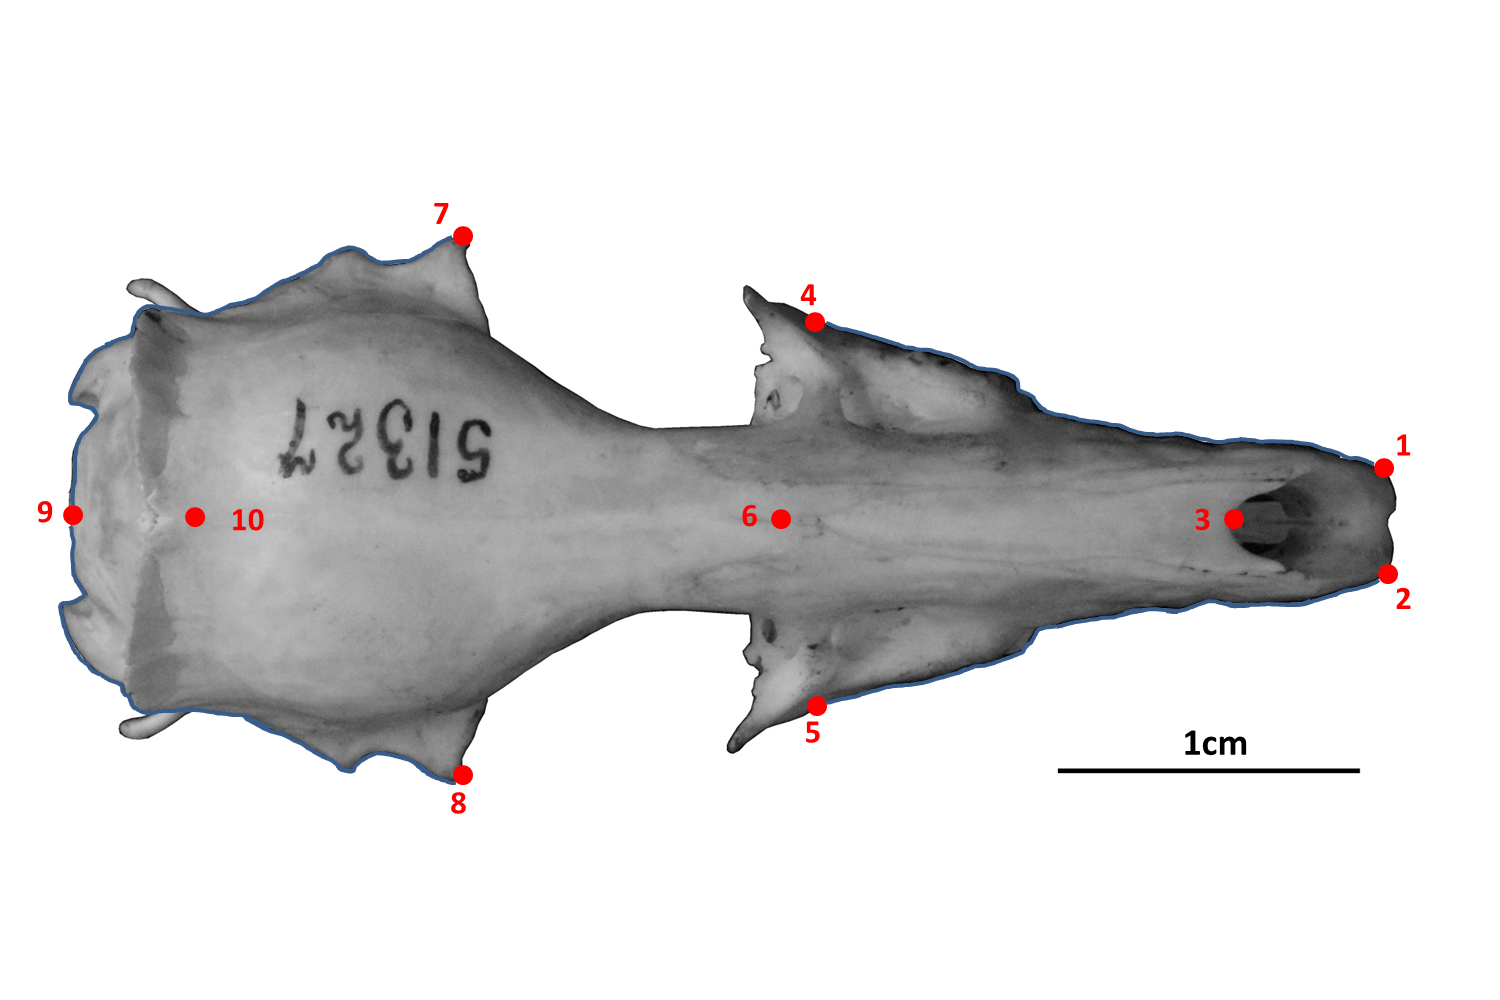
\includegraphics[width=1\linewidth]{Methods/figures/AMNH_51327_dorsallandmarksdiagram.png}
\caption[Skulls: dorsal landmarks]
{Landmarks (red) and curves (blue) for the skulls in dorsal view. Curves were re-sampled to the same number of evenly-spaced points. See table \ref{tab:skdors} for description of curves and landmarks.\textit{Potamogale velox} (Tenrecidae) skull, museum accession number: AMNH\_51327}
\label{fig:skdors_landmarks}
\end{figure}


\begin{table}[h]
\caption[Skulls: dorsal landmarks]
		{Descriptions of the landmarks (points) and curves (semilandmarks) for the skulls in dorsal view (figure \ref{fig:skdors_landmarks})} 
%Skdors landmarks

\begin{tabular}[t]{p{3cm}  l}		
\hline
\textbf{Landmark} & \textbf{Description} \\
\hline
%------------------------------------------------------------
1 + 2 & Left (1) and right (2) anterior points of the premaxilla \\
%------------------------------------------------------------
3 & Anterior of the nasal bones in the midline \\
%------------------------------------------------------------
4 + 5 &	Maximum width of the palate (maxillary) on the left (4) and right (5)\\
%------------------------------------------------------------
6 & Midline intersection between nasal and frontal bones \\
%------------------------------------------------------------
7 + 8 & Widest point of the skull on the left (7) and right (8) \\
%------------------------------------------------------------
9 &	Posterior of the skull in the midline \\
	%Panchetti 2008 and Macholan2008 have different definitions for this one so I need to choose one
%------------------------------------------------------------
10 & Posterior intersection between saggital and parietal sutures \\
%--------------------------------------
\hline
\textbf{Curve A} & Outline of the braincase on the left side, between landmarks 9 and 7\\ 
(12 points) & (does not include visible features from the lower (ventral) side of the skull) \\

\textbf{Curve B} & Outline of the palate on the left side, between landamarks 4 and 1 \\
(10 points) & (outline of the rostrum only, not the shape of the teeth)\\

\textbf{Curve C} &	Outline of the braincase on the right side, between landmarks 9 and 8 \\
(12 points) & (does not include visible features from the lower (ventral) side of the skull) \\

\textbf{Curve D} & Outline of the palate on the right side, between landamarks 5 and 2 \\
(10 points) & (outline of the rostrum only, not the shape of the teeth)\\
%------------------------------------------------------------
\hline
\end{tabular}
\label{tab:skdors}
\end{table}
%=======================================================================

\subsection{\normalfont{Mandibles}}
I placed seven landmarks and drew four curves on each mandible picture (again, reflecting any pictures of the left mandible so they could be compared to pictures of the right side). I drew separate curves around each of the three processes of the ascending ramus; coronoid, condyloid and angular and along the base of the horizontal ramus of the jaw. While obviously part of an integrated jaw unit, the development of the mandibular processes are also, in some aspects, independent since they attach different muscles which exert different masticatory forces on the jaw \citep{Barrow2008}. Therefore, by drawing separate curves around each of these elements, my ensuing analyses could assess the relative shape changes of different components of the jaw with relevance to variation in feeding strategies and capabilities.
%********
%Why do we care about independence??
%I don’t like how I’ve phrased the above paragraph but I just thought it was a nice point in the Barrow paper so I want to include it somewhere.
%********

%Mandibles' landmarks
\begin{figure}[H]
\centering
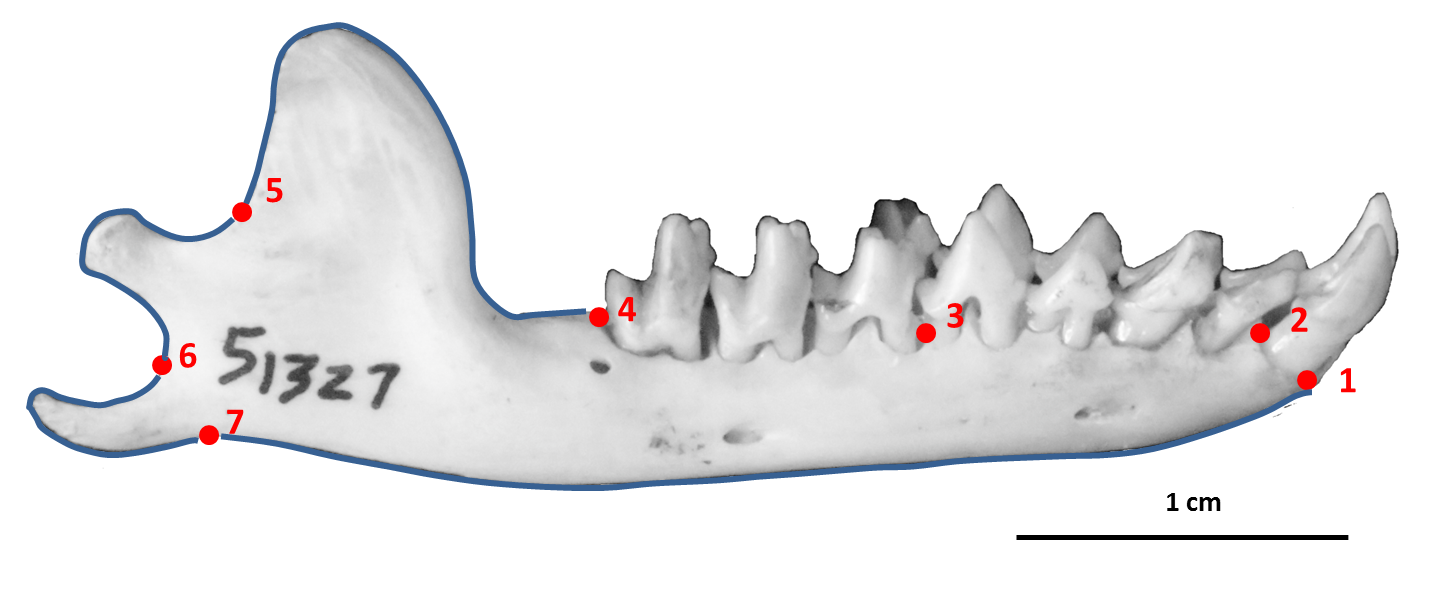
\includegraphics[width=1\linewidth]{Methods/figures/AMNH_51327_landmarksdiagram.png}

\caption[Mandibles' landmarks]
{Landmarks (red) and curves (blue) used for the mandibles. Curves were re-sampled to the same number of evenly-spaced points. See table \ref{tab:mands} for description of curves and landmarks.\textit{Potamogale velox} (Tenrecidae) mandible, accession number: AMNH\_51327}
\label{fig:mands_landmarks}
\end{figure}

\begin{table}[h]			
\centering
\caption[Mandibles' landmarks]
	{Descriptions of the landmarks (points) and curves (semilandmarks) for the mandibles in lateral (buccal) view (figure \ref{fig:mands_landmarks}}
%Mandibles landmarks


\begin{tabular}[t]{p{0.2\textwidth} p{0.75\textwidth}}		
\hline
\textbf{Landmark} & \textbf{Description} \\
\hline
1 & Anterior of the alveolus of the first incisor \\
2 & Posterior of the alveolus of the first incisor \\
3 &	Anterior of the alveolus of the first molar \\
4 & Posterior of the alveolus of the last molar \\
5 & Maximum curvature between the coronoid and condylar processes\\
6 & Maximum curvature between the condylar and angular processes  \\
7 &	Maximum curvature between the angular process and the horizontal ramus \\
%---------------------------------------------------
\hline
Curve A & Condyloid process (between landmarks 4 and 5, 15 points)\\
Curve B & Condylar process (between landmarks 5 and 6, 15 points) \\
Curve C & Angular process (between landmarks 6 and 7, 15 points)  \\
Curve D & Base of the jaw (between landmarks 7 and 1, 12 points)  \\
%---------------------------------------------------
\hline
\end{tabular}
\label{tab:mands} %give it a label so I can refer to it in the text
\end{table}
%===================================================

\subsection{\normalfont{Skins}}
% Outline analysis of skins for overall body shape?

%####################################################
\section{Error checking}
My data are prone to a number of different error sources. These include 1) taxonomic identification which has not been updated to currently accepted terms, 2) specimen ID errors, 3) possible variation associated with sex and age class of individuals, 4) the accuracy and repeatability with which species traits are measured, 5) morphometric errors associated with photographing specimens and the placement of landmarks. I address each of these possible sources of error below.  

\subsection{\normalfont{Taxonomic}}
I recorded species names as they were written on museum specimen labels and then corrected them to match the taxonomy Wilson and Reader’s Mammal Species of the World \citeyearpar{Wilson2005}. For recently identified species, such as \textit{Microgale jobihely} \citep{Goodman2006}, which are not included in Wilson and Reader \citeyearpar{Wilson2005}, I used the taxonomy recorded on the labels. 

\subsection{\normalfont{Specimen ID}}
	%add in Natalie's centroid means?
	
There were four specimens from the Smithsonian Institute which had species labels which did not match between skulls and skins with the same specimen ID numbers. The four skulls were labelled as \textit{Hemicentetes semispinosus}. The corresponding skins were originally labelled as \textit{H. semispinosus} but this was crossed out and changed to \textit{H. nigriceps}. The re-labelled skins looked clearly different to the undisputed \textit{H. semispinosus} skins and also look more similar to other pictures of \textit{H. nigriceps}. Therefore, I made the assumption that the re-labelling of the skins as \textit{H. nigriceps} represents the true taxonomy and I treated the corresponding skulls as \textit{H. nigriceps}.

\subsection{\normalfont{Specimen sex and age}}
I included both male and female specimens in my data as significant sexual dimorphism in skull or body size has not been identified in any of my species \citep[NEED MORE REFERENCES][]{Olson2004}.
%***********************
%Need to do a test of male vs. female??
%*********************************

Information about the sex and/or age of an individual is often missing from museum records. Mammalian species can often be identified as juveniles by looking for incomplete fusion of the crania and non-fully erupted dentition (REFS) However, age classification in tenrecs is difficult using these criteria; in some species, the last molar does not erupt fully until the first molar has been shed so the full dentition is never present at any one time \citep{Nowak1983}. It is also difficult to distinguish deciduous from permanent teeth in \textit{Microgale} tenrecs \citep{Asher2008} which has led to confusion and misidentification of juvenile forms as separate species \citep{Olson2004}. I excluded any obvious juvenile specimens from my data set. Where specimens could not be obviously identified as juveniles I treated them all as equivalent adult forms. 
%******************************
%(Check the Potamogale against the other Potamogales?? Keep the _sp for family or genus level analyses but exclude from species-level things)
%******************************

\subsection{\normalfont{Linear measurements}}
As mentioned above, I took three replicate measurements of most of my variables and five replicates of other variables. Some morphometric studies take replicate measurements of a trait and use the average value for further analyses. 
%(is this true? check papers) 
Rather than taking the mean of each of three (or five) measures, I used the median as it is less likely to be skewed by outliers and gives a more accurate representation of the true value of the trait.
Before extracting the median values I followed the protocol for assessing measurement error outlined by \citep{Cooper2009}. This method assesses whether there is a reasonable correlation among the replicate measurements of the same variable. The error checking criteria are based on two calculations; the coefficient of variation and the percentage spread.
I calculated the coefficient of variation (standard deviation/mean*100) for each measurement. This value estimates the extent to which replicate measurements deviate from the mean. When the coefficient of variation was less than 5\%, I accepted the median value as an accurate measurement of the size of the structure. 
If the coefficient of variation was greater than 5\%, indicative of a low agreement between replicate measurements, I measured the percentage spread of the data. For variables measured three times, I calculated percentage spread as [(minimum difference between neighbouring measurements)/ (range of measured values)*100].
For variables that were measured five times, the differences between neighbouring values were calculated and labelled from smallest to largest as a, b, c, and d with the range of the measured values designated as e \citep{Cooper2009}. For these variables, I calculated percentage spread as [(a/e + b/e + c/e)*100]. 
Small percentage spread values indicate close agreement between repeated measurements. When percentage spread approaches 50\% the data are evenly spread out and therefore there is no way of knowing whether the median value is an accurate measurement of the trait \citep{Cooper2009}. I chose to use to use 25\% as a cut off point for accepting the accuracy of measured traits.

I used these error checking criteria to assess the accuracy of my repeated measurements of both skulls and limbs. 
%***********************************
%(I need to present all of this as more of a narrative but keep the detail in for the moment.)
%***********************************
Of the 20 measurements for xxx skulls, there were xx variables belonging to xx skulls which had coefficient of variation > 5\% and percentage spread >25 \%. My final skull data set included xx replicates of xx variables from xx specimens comprising xx species.

Of the 19 measurements for xxx limbs, there were xx variables belonging to xx specimens which had coefficient of variation > 5\% and percentage spread >25 \%. My final limb data set included xx replicates of xx variables from xx specimens comprising xx species.

\subsection{\normalfont{Landmark morphometrics}}

I used 2D morphometrics to compare the morphologies of the skulls. The small size of my specimens, combined with the number of specimens involved in my study made 3D imaging impractical. It takes roughly 1.5 hours for a good quality scan of each specimen so it would take XX hours to compile a useful data set. While 2D methods are an accepted means of comparing morphological shape \citep[e.g.][]{Adams2004, Mitteroecker2009}, particularly for comparing skull morphologies of small mammals \citep[e.g.][]{Cardini2003, Panchetti2008, White2008, Barrow2008, Scalici2011}, the inherent discrepancies associated with comparing three dimensional objects using two dimensional pictures do introduce some difficulties of possible distortion of the image \citep{Arnqvist1998}. Similarly, human error with how landmarks are positioned on specimens could also introduce noise into further analyses. In contrast to detailed intraspecific work (REFS) photographic or landmark placement errors are unlikely to be significant in interspecific studies since one would expect that the morphological variation among species is large enough to  be detected as a signal above any background noise associated with methodological error (REFS). Nevertheless, it is still important to assess measurement error in a morphometric data set to increase confidence in the outcome of final analyses.
I identify two main sources of morphometric measurement error; specimen orientation and placement of landmarks.

%***************************
%NB: I never actually completed these error checking analyses so I need to go back and do it again
%********************************

\subsection{\normalfont Specimen orientation}

Variation in the orientation of specimens for photography is one of the main sources of error in 2D morphometric studies \citep{Adriaens2007}. If specimens are not placed on a flat plane or in a consistent position relative to the camera, areas of the object which are tilted towards the camera will appear to be larger than reality, distorting any subsequent morphometric analyses of the shape. 
I used a random subset of skulls comprised of one representative from each of my 89 species 
%*******************************************
%(probably don’t need to use this many for error checking but how should I choose which ones to include?) 

to estimate the overall specimen orientation error in my photographic dataset. This subset included representatives from each tenrec and golden mole species along with samples from my comparative species (total of xx moles, xx shrews, xx hedgehogs…)  I took three sets of pictures of each view of the skulls and mandibles, cycling through the pictures so that the specimen was removed and re-positioned before every shot \citep{Viscosi2011}. 
%********I need to add more here

\subsection{\normalfont{Landmark placement}}

I placed the landmarks on each set of pictures so inter-observer variation is not an issue for my study.  However, repeatability and reliability of my choice of landmarks could affect the final results of my analyses \citep{Arnqvist1998}.
I used a combined, nested approach to test for both orientation and landmark placement error \citep{Arnqvist1998, Barrow2008}. For each of the 89 specimens in my random subset of species, I photographed their skulls (dorsal, ventral and lateral views) and mandibles three times. I then copied these images and placed landmarks on 3 copies of each image. I used a nested mixed mode ANOVA to assess the measurement error of the Procrustes-superimposed coordinates. There were three factors in my ANOVA; specimen, photo (3 pictures of each specimen) and landmark trial (placed landmarks on 3 copies of each of my photos).


%Effect size for the variance explained by each factor, based on inter landmark linear distances……..
%(I could also use PC scores or a Mahalanobis distance matrix…)

\section{Summary of the morphological data set}

\section{Ecological data}


